\documentclass{scrreprt}

\usepackage{aligned-overset}
\usepackage{amsmath}
\usepackage{amssymb}
\usepackage{bm}
\usepackage[shortlabels]{enumitem}
\usepackage{hyperref}
\usepackage[utf8]{inputenc}
\usepackage{mathtools}
\usepackage{physics}
\usepackage{tabularx}
\usepackage{titling}
\usepackage{fancyhdr}
\usepackage{xfrac}
\usepackage{pgfplots}

\pgfplotsset{compat = newest}
\usepgfplotslibrary{fillbetween}

\author{}
\date{SoSe 2021}
\title{Hausaufgabe 08 \\Analysis - Weiterführende Konzepte}

\setlength{\headheight}{26pt}
\pagestyle{fancy}
\fancyhf{}
\lhead{\thetitle}
\rhead{\theauthor}
\lfoot{\thedate}
\rfoot{Seite \thepage}

\begin{document}
\paragraph{Hausaufgabe 2} Gegeben sei die Funktion
$f \colon \mathbb{R}^2 \to \mathbb{R}$ mit
\begin{flalign*}
  f(x) &\coloneqq \begin{cases}
    \frac{x_1x_2}{\sqrt{x_1^2 + x_2^2}}, & \text{für } x = \qty(x_1, x_2) \ne (0, 0) \\
    0, & \text{für } x = (0, 0)
  \end{cases} &
\end{flalign*}
\begin{center}
  \resizebox{.8\textwidth}{!}{
    \begin{tikzpicture}[
        declare function={
          f(\x, \y) = \x^2 + \y^2 != 0 ? (\x*\y)/(sqrt(\x^2 + \y^2)) : 0;
        }
      ]
      \begin{axis}[
        xlabel = $x$,
        ylabel = $y$,
        view={20}{40},
      ]
        \addplot3[
          surf,
          domain=-1:1,
          samples=25,
          shader=faceted interp,
        ] {f(x, y)};
      \end{axis}
    \end{tikzpicture}
  }
\end{center}

\begin{enumerate}[a)]
\item Zeigen Sie, dass $f$ in $(0, 0)$ stetig ist.
  \subparagraph{Lösung:} Die Funktion $f$ heißt stetig im Punkt
  $x_0 = (0, 0) \in \mathbb{R}^2$, wenn
  \begin{flalign*}
    \forall \epsilon > 0 \:\exists\: \delta > 0 \forall y \in \mathbb{R}^2 \colon \norm{x_0 - y}_2 < \delta
    &\Rightarrow \abs{f(x_0) - f(y)} < \epsilon & \\
    \sqrt{y_1^2 + y_2^2} < \delta &\Rightarrow \abs{\frac{y_1y_2}{\sqrt{y_1^2 + y_2^2}}} < \epsilon \\
    \sqrt{y_1^2 + y_2^2} < \delta &\Rightarrow \frac{\abs{y_1y_2}}{\sqrt{y_1^2 + y_2^2}} < \epsilon \\
    \sqrt{y_1^2 + y_2^2} < \delta &\Rightarrow \sqrt{y_1^2 + y_2^2} \cdot \frac{\abs{y_1y_2}}{y_1^2 + y_2^2} < \epsilon \\
    \sqrt{y_1^2 + y_2^2} < \delta &\Rightarrow \sqrt{y_1^2 + y_2^2} \cdot \frac{1}{\abs{\frac{y_1}{y_2}} + \abs{\frac{y_2}{y_1}}}
    \leq \frac{\sqrt{y_1^2 + y_2^2}}{2} < \epsilon
  \end{flalign*}
  $\Rightarrow f$ ist im Punkt $(0, 0)$ stetig mit $\delta > 2\epsilon$.

\newpage
\item Zeigen Sie, dass die partiellen Ableitungen $f$ in $(0, 0)$ existieren.
  Existiert die Richtungsableitung von $f$ in $(0, 0)$ in Richtung von
  $v = \frac{1}{\sqrt{2}}\qty(e_1 + e_2) = \frac{1}{\sqrt{2}(1, 1)}$?
  Warum ist $f$ in $(0, 0)$ nicht differenzierbar?

  \subparagraph{Lösung:} Für $t \in \mathbb{R}$ gilt
  $g(t) = f(t, 0) = 0 = f(0, t)$.z
  Folglich ist
  \begin{flalign*}
    \frac{\partial^nf(0,0)}{\partial x_1^n} &=
    \frac{\partial^n f(0, 0)}{\partial x_2^n} = g^{(n)}(0) = 0
    \text{ für alle } n \in \mathbb{N}
  \end{flalign*}

  Die Funktion $f$ heißt in $x = (0, 0) \in \mathbb{R}^2$ in Richtung
  $v = \frac{1}{\sqrt{2}(1, 1)}$ differenzierbar, falls die Funktion
  \[
    k \colon ]-r, r[ \to \mathbb{R}, t \mapsto f(x + t \cdot v)
  \]
  (für $r > 0$ klein genug) in $0$ differenzierbar ist und dann heißt
  \[
    \frac{\partial f}{\partial v}(x) \coloneqq \lim_{t \to 0} \frac{k(t) - f(x)}{t}
  \]
  die Richtungsableitung von $f$ im Punkt $(0, 0)$ in Richtung $v$.

  \[
    k(t) = f((0,0) + t \cdot v) = f\qty(\frac{t}{\sqrt(2)}, \frac{t}{\sqrt(2)})
    = \begin{cases}
      \frac{\sfrac{t^2}{2}}{\sqrt{2\sfrac{t^2}{2}}} = \frac{t}{2} & t \ne 0 \\
      0 & t = 0
    \end{cases}
  \]
  Da für $t = 0$ der Wert von $\frac{t}{2} = k(0)$ entspricht, gilt
  $k(t) = \frac{t}{2}$.
  $\Rightarrow$ die Richtungsableitung von $f$ im Punkt $(0, 0)$ in Richtung
  $v$ existiert mit
  \[
    \frac{\partial f}{\partial v}(x) \coloneqq \lim_{t \to 0} \frac{k(t) - f(x)}{t}
    = \lim_{t \to 0} \frac{\sfrac{t}{2} - f((0,0))}{t} = \frac{1}{2}
  \]
\end{enumerate}

\end{document}